\section{Calibration and Event Reconstruction}
\subsection{Gain Calibration of PMTs} 
We use ET 9823QKB photomultipliers that have a dark current up to 1000 nA as specified by the manufacturer. At a nominal high voltage of around $\sim$ 2,400 V, it was impossible to observe a single photoelectron peak due to the high dark noise rate. Therefore we developed a special procedure for the gain calibration of the PMTs. We have implemented a method of fitting and extracting the position of the single photoelectron peak using the parametrization described in [“Absolute calibration and monitoring of a spectrometric channel using a photomultiplier” Bellamy et al. NIM A 339 468-476]. \\ 

\begin{comment}
The fast, stable light source (see section 6) is the core component of the HTCC Light Monitoring System (LMS). It was designed and built exclusively for reliably calibrating the gain of PMTs. The LED light is distributed relatively evenly via an 4" of diameter integrating sphere and fiber optics. The PMT signals illuminated by a light source (an array of LED lights) have timing parameters very close to the timing of the dark noise signals. In fact, the signal from an LED light mimics that of the signal from the detector. Since LMS allowed us to generate light pulses of variable intensity and frequency it became possible to observe the PMT response (which was well separated from the exponential dark noise background). \\
\indent Via analysis of PMT response spectra obtained with a constant intensity of an LED light at a fixed frequency we were able to extract the  position of single photoelectron peak in cases when the average intensity of light (which is fluctuating) impinging the PMT photocathode is as low as on the order of a few photoelectrons. In the Fig.\ref{fig:WILLIAM_1} the main definitions are presented. 
\end{comment}
 
 \indent Fig. \ref{fig:WILLIAM_1} shows the main definitions of analysis of a representative PMT response obtained with LMS to extract the  position of a single photoelectron peak when the average intensity of the LMS light is about few photoelectrons. 

\begin{figure}[!h]
    \centering
    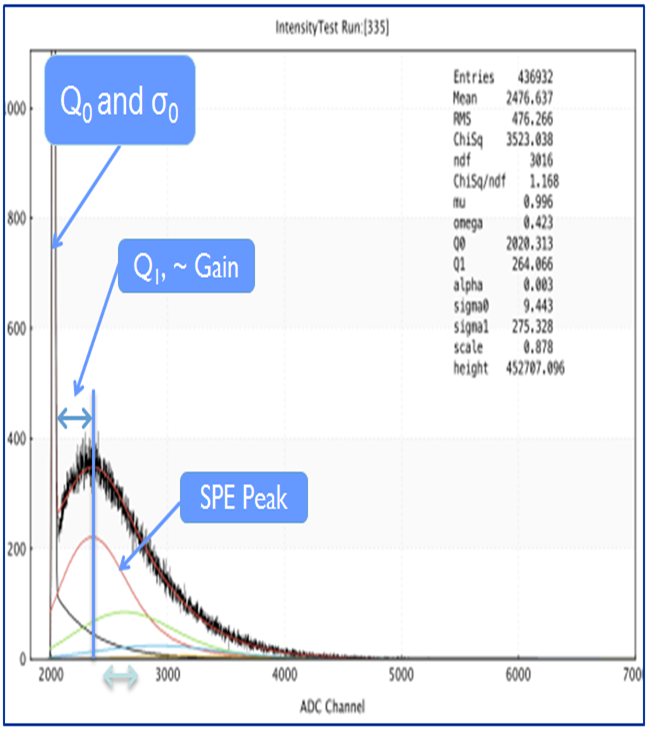
\includegraphics[width=1.0\linewidth,trim={0.0cm 0.0cm 0.0cm 0.0cm},clip]{images/WILLIAM_1.png}
    \caption{Definitions: $Q_{o}$ and $\sigma_{o}$ are the position and width of the pedestal, $Q_{ 1}$ is proportional to the gain of the PMT. The red curve defines a single photoelectron peak. The green and blue curves describe 2 and 3 photoelectron peak.}
    \label{fig:WILLIAM_1}
\end{figure}

Fig. ~\ref{fig:WILLIAM_2} shows an example of typical fits of the PMT response to LMS light of constant intensity at different high voltages. The corresponding dependence of the single photoelectron peak position as a function of high voltage is given in Fig. \ref{fig:WILLIAM_3_NEW}. Of course this method required that LMS generate light pulses of stable intensity. The results of the single photoelectron peak position can be used for gain matching. Calibration measurements are performed for all PMTs in parallel at the same LMS settings. This can be done by adjusting the high voltage applied to individual channels.

\begin{figure*}[ht]
\centering
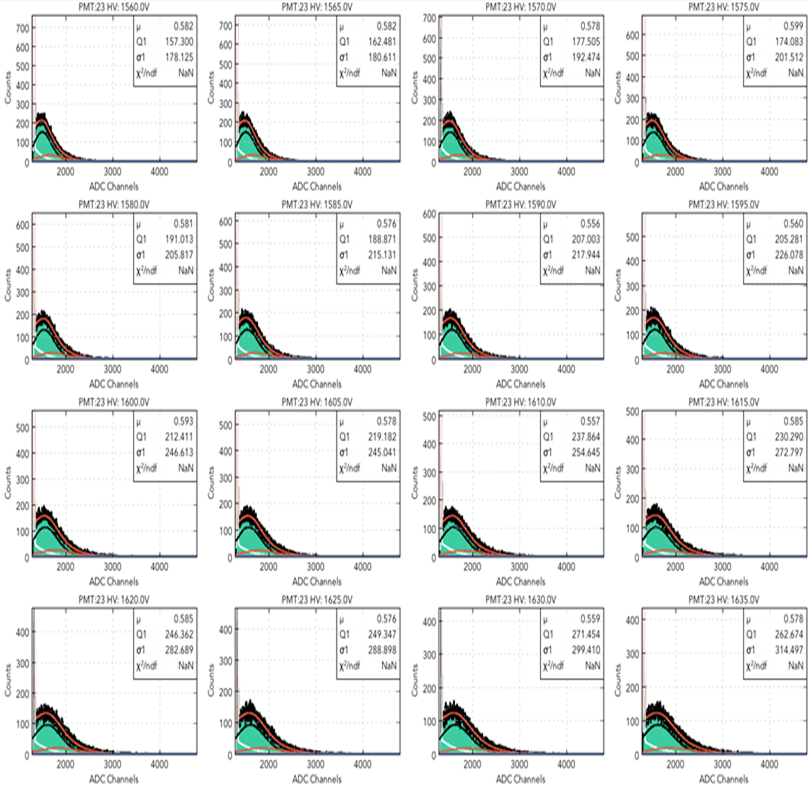
\includegraphics[width=0.99\linewidth]{images/WILLIAM_2.png}
\caption{Response of representative PMT to LMS light of constant intensity at high voltage changing from 1560 V to 1635 V with 5 V increment.}
\label{fig:WILLIAM_2}
\end{figure*}

\begin{figure}[ht]
\centering
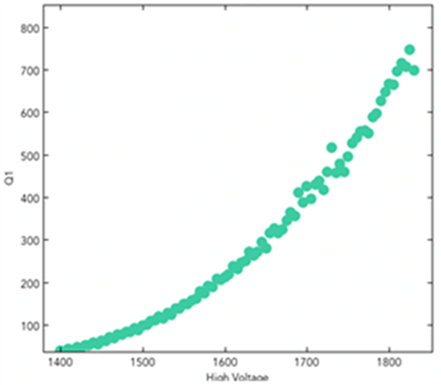
\includegraphics[width=0.99\linewidth]{images/WILLIAM_3_NEW.png}
\caption{Single photoelectron peak position as a function of high voltage for a representative HTCC PMT.}
\label{fig:WILLIAM_3_NEW}
\end{figure}

The distinguishing feature of the HTCC LMS is that the observed repeatability of results is within 5-10\% of that obtained in runs at different but stable light intensities and frequencies. This is demonstrated in Fig. \ref{fig:WILLIAM_5} where are given the positions of the single photoelectron peak at different LMS light intensities shown for a representative PMT at a fixed voltage setting. The fitting function is stable across a wide range of intensities and accurately describes PMT response at low intensities ($\mu<1.0$). The position of the peak stays within 5\% of the mean. Consequently there is no need to keep the light source intensity uniform, i.e. stay the same or close to the same in different calibration runs that are taken whenever necessary.

\begin{figure}[ht]
\centering
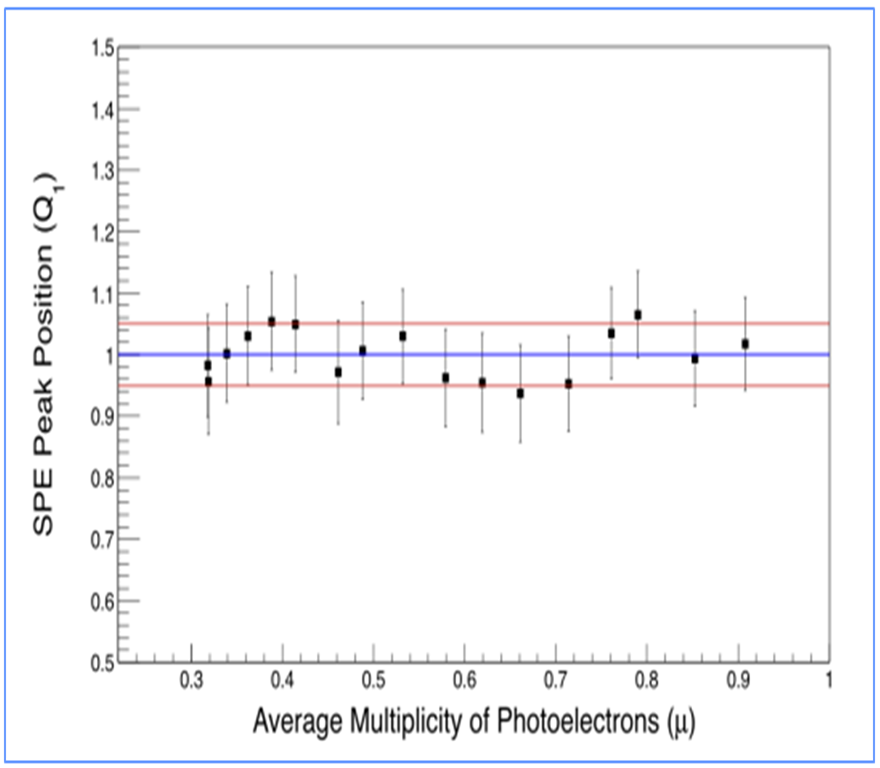
\includegraphics[width=0.99\linewidth]{images/WILLIAM_5.png}
\caption{Single photoelectron peak position as a function of LMS light intensity at constant high voltage for a representative HTCC PMT. Red lines show 5\% deviation, blue line-averaged single photoelectron peak position.}
\label{fig:WILLIAM_5}
\end{figure}

\begin{comment}
Runs were taken at constant high voltage, i.e. $Q_{ 1}$, with changing LED light intensity ($\mu$). These runs were fit in batch mode with the production fitter and all runs have good $\chi{^2}$.
\end{comment}

We have compared our preliminary single photoelectron calibration results with results obtained using [Degtiarenko]. The same PMT with modified divider was tested. Each data set was normalized by the average value. Fig. \ref{fig:WILLIAM_4} shows the results for the 12 PMTs monitoring events in the polar angle range from $27.5^\circ$ to $35^\circ$ (Ring 4) from 6 sectors. Both approaches are providing close results whereas external light sources and software used in calibration measurements were different.

\begin{figure}[ht]
\centering
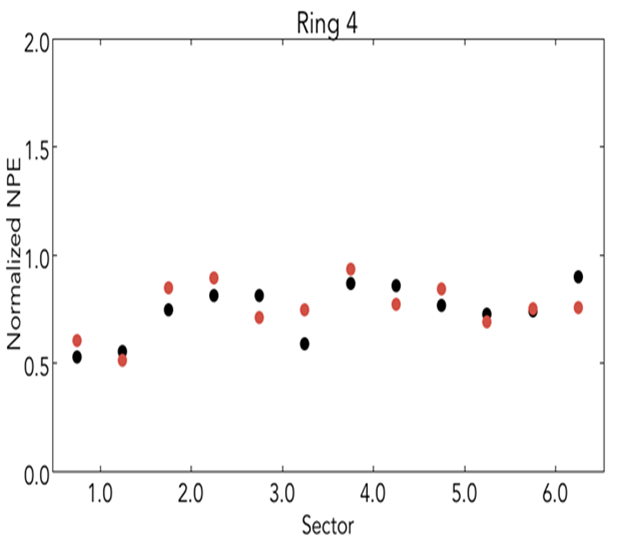
\includegraphics[width=0.99\linewidth]{images/WILLIAM_4.png}
\caption{Comparison of preliminary calibration results using two different fitting codes: [B] (black dots) and [D] (red dots).}
\label{fig:WILLIAM_4}
\end{figure}

\subsection{Response Equalization} Different factors (including imperfections of the mirror working surface, dust deposition, condensation of fumes, overall mirror shape distortions, and gain instability of the individual PMTs) can lead to a variation in the signal strength from the individual channels---even after comprehensive single photoelectron calibration is complete. These variations should be corrected independently of their physical origin, as the trigger efficiency is heavily dependent on the uniformity of the HTCC response. In the beginning of every physics run period we analyze the first data in order to estimate the signal strength in each of the 48 channels. We then develop corresponding correction factors, which align the signals between individual channels to the average value between channels. These correction factors are then propagated to both the offline reconstruction (CLAS Calibration Data Base, or ccdb) and online trigger gain files. In the Fig.~\ref{fig:NICK_svodni} are shown results on channels response before and after equalization.

\begin{comment}
Fig.~\ref{fig:htccSinglePmtResponce} shows an example of the aligned response of the HTCC.

\begin{figure*}[ht]
\centering
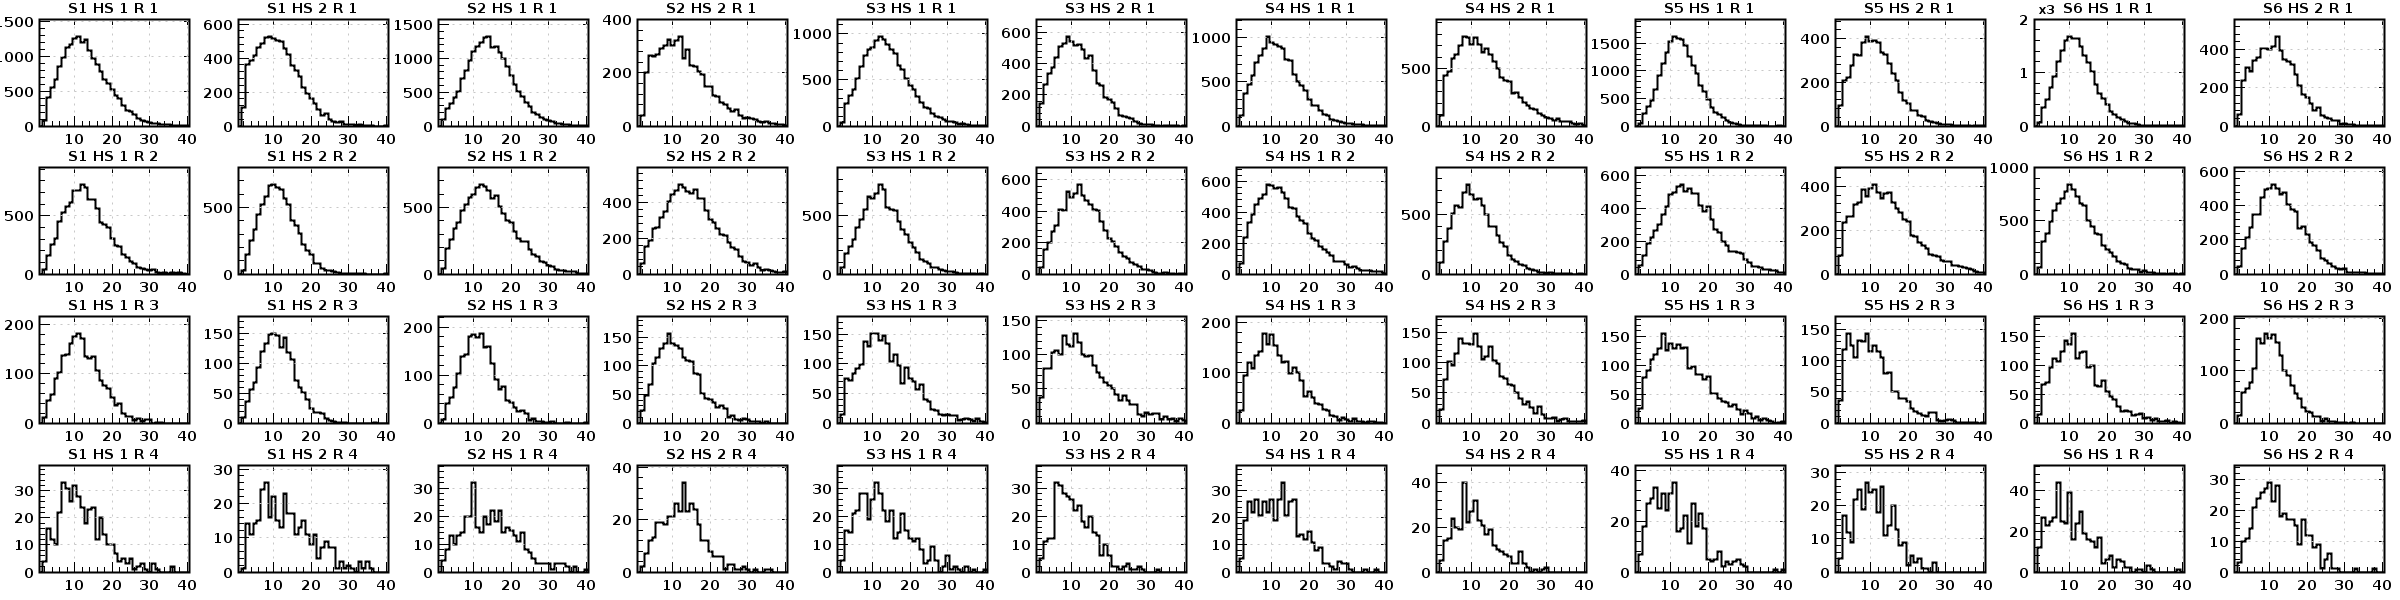
\includegraphics[width=0.99\linewidth]{images/nphePMT6595.png}
\caption{Response of all 48 PMTs to the single-hit events after response equalization. Top row correspond to Ring One (closest to the beam-line), next one is Ring Two and so on. Number of events drops significantly as we move toward the outer rings.}
\label{fig:htccSinglePmtResponce}
\end{figure*}
\end{comment}



\begin{figure}[ht]
\centering
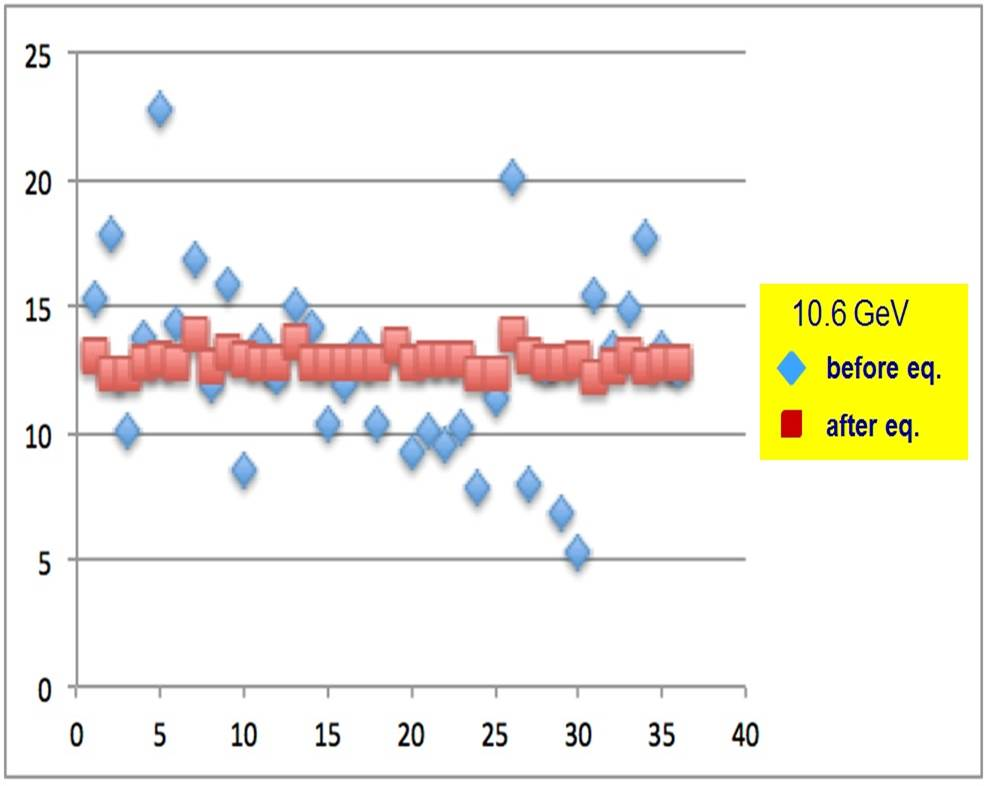
\includegraphics[width=0.99\linewidth]{images/NICK_svodni.jpg}
\caption{Response of PMTs before and after response equalization.}
\label{fig:NICK_svodni}
\end{figure}

\subsection{Timing Calibration} Since the HTCC is the part of the trigger, it is required that the timing of the individual channels is aligned to aid the online cluster reconstruction. As a result, the timing calibration of the HTCC is done in two steps: the first step is performed on the level of the FADC, and the second step (finer step) is done in the offline calibration. \\
\indent The online calibration is done using the independent trigger from the Forward Tagger, [Ref. FT]. Timing of all 48 HTCC channels is aligned in the FADC configuration files by setting the appropriate delays with a precision of 4 ns (the best available using the FADC). Since the timing resolution of individual channels is on the order of about 1 ns we can achieve better resolution of the detector than the 4 ns available from the FADC. To do so, we calculate the time at the vertex for each of 48 channels and estimate the time shift between the individual channels. These time shifts are added to the ccdb and are applied at the reconstruction stage. Fig.~\ref{fig:htcccombinedTimingResponce} shows the timing resolution combined over all 48 PMTs which is on the level of 0.6 ns.
\begin{figure}[ht]
\centering
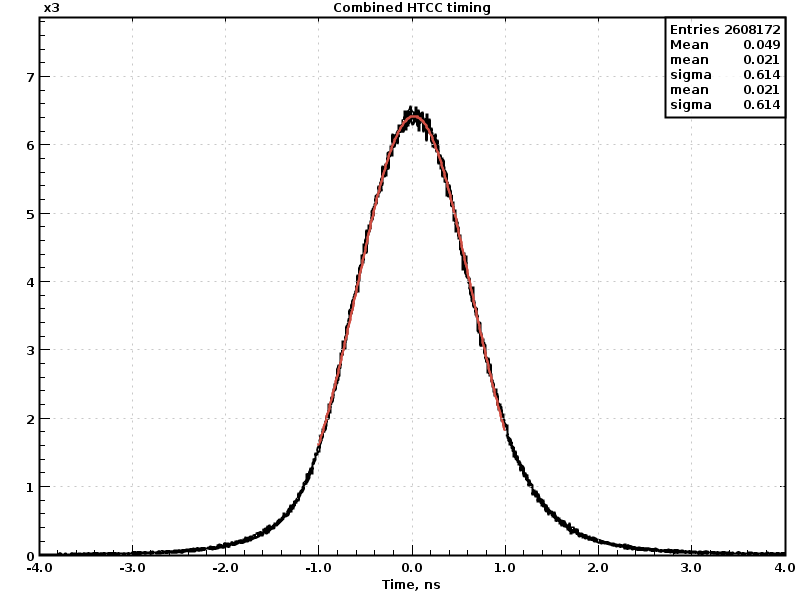
\includegraphics[width=0.95\linewidth]{images/deltaTime6.png}
\caption{Combined timing of the 48 HTCC PMTs.}
\label{fig:htcccombinedTimingResponce}
\end{figure}

\subsection{Event Reconstruction} The goal of the reconstruction procedure is to reconstruct the real signal strength, time, and hit position from the raw ADC signals. This is done in two steps:

\begin{enumerate}
    \item In the decoding stage: the signal is converted from the hardware notation (crate, slot, channel) into the CLAS12 notation (sector, layer, component). For each signal, its amplitude (in ADC channels) and timing is determined from the threshold crossing, and the pedestal is subtracted. The pedestal value for each channel is determined during special pedestal runs and is stored for both trigger and offline reconstruction purposes.
    \item In the reconstruction stage: the ADC signal is converted into the number of the photoelectrons using the gain constants in the CLAS calibration database ($ccdb$). The physical design of the HTCC allows the Cerenkov radiation from one electron to split into up to four channels (see Fig.~\ref{fig:htccClustersSplit}). In order to reconstruct the signal strength, we need to combine such split signals into a single cluster. We start by selecting the strongest hit for a given event and use it as the starting point of the cluster. We then look for adjacent hits within a certain time window (stored as a parameter in the $ccdb$). If such hits are found, they will be added to the cluster. In the final stage, the signal strength is determined as the sum of the individual signals, and the signal time is determined as the average between the individual signals, weighted by the corresponding number of the photoelectrons. The hit angular coordinate is determined as the average between the individual hits forming the cluster. Hits, attributed to the established clusters, are removed from further consideration, and the algorithm continues to look for the next cluster until the list of hits is exhausted.

\begin{figure}[ht]
\centering
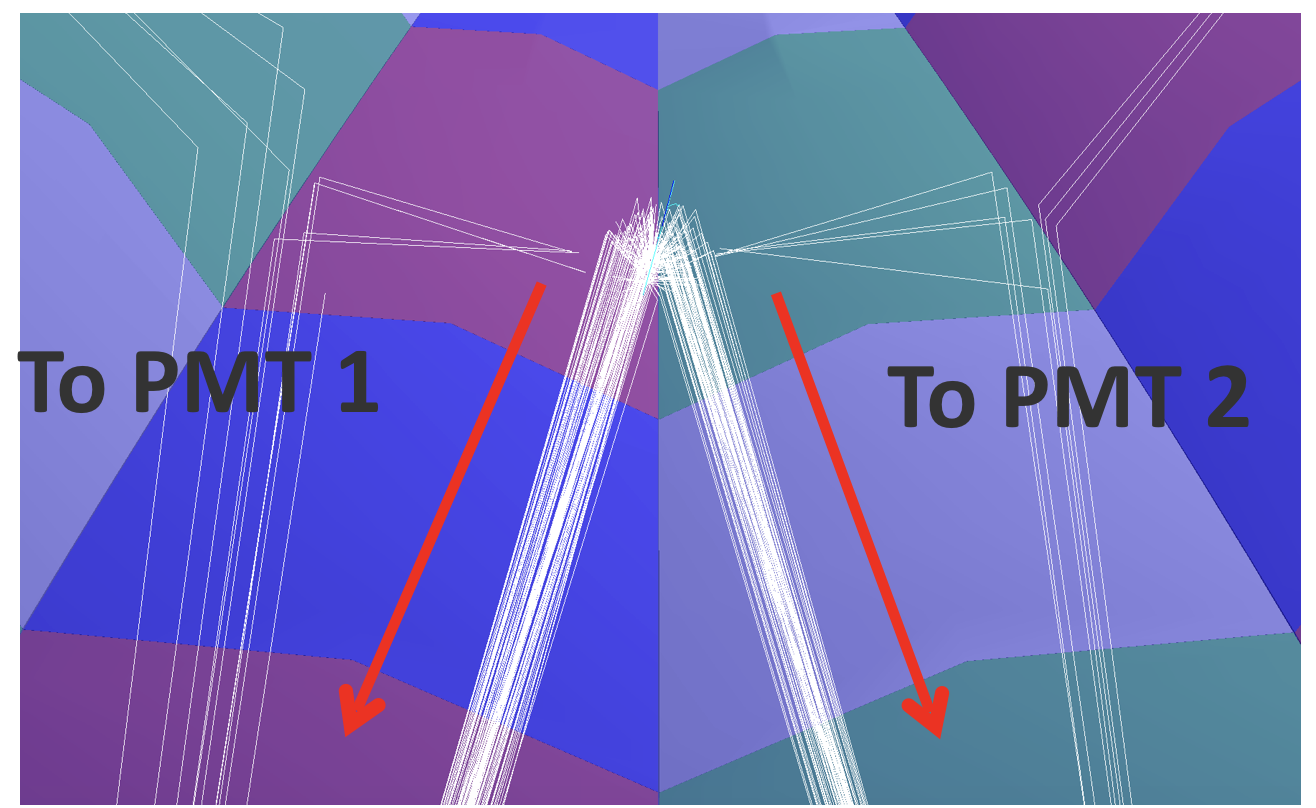
\includegraphics[width=0.95\linewidth]{images/htccClustersSplit.png}
\caption{Splitting of the Cerenkov radiation between two mirrors. Geometrically the signal can split into up to four mirrors.}
\label{fig:htccClustersSplit}
\end{figure}
\end{enumerate}
